% =============================================================================
% ReBel: Rescuing Step-Level Credit Assignment via Belief-Enhanced Grouping
% NeurIPS 2026 — Experiments Chapter
% =============================================================================
% Compile with: pdflatex + bibtex
% Requires: booktabs, multirow, graphicx, subcaption, amsmath, xcolor
% =============================================================================

\section{Experiments}
\label{sec:experiments}

We evaluate ReBel on two challenging multi-step interactive environments:
ALFWorld~\citep{shridhar2021alfworld}, a text-based household task benchmark,
and WebShop~\citep{yao2022webshop}, a web-based e-commerce navigation benchmark.
Our experiments address four questions:
\textbf{(Q1)}~Does ReBel outperform episode-level and existing step-level baselines?
\textbf{(Q2)}~What is the individual contribution of each component?
\textbf{(Q3)}~How does HiBO address the singleton group problem in observation-based grouping?
\textbf{(Q4)}~Does the adaptive differential decay resolve the reward shaping bias?


% -----------------------------------------------------------------------------
\subsection{Experimental Setup}
\label{sec:exp_setup}

\paragraph{Environments.}
\textbf{ALFWorld}~\citep{shridhar2021alfworld} comprises six household task types
(pick-and-place, pick-two, pick-heat, pick-cool, pick-clean, look-at-object)
requiring 8--30 interaction steps.
We use 16 training prompts per batch and evaluate on the full 128-task validation set
at generalization level~0 (seen room layouts).
\textbf{WebShop}~\citep{yao2022webshop} requires an agent to navigate a simulated
e-commerce website through \texttt{search[...]} and \texttt{click[...]} actions to
purchase a product matching a natural language instruction.
Episodes last up to 15 steps and yield a continuous reward $r \in [0,1]$ based on
attribute, option, and price matching.
Both environments expose a text observation at each step, from which the agent must
select a valid action.

\paragraph{Base model and cold-start.}
All methods start from the same supervised fine-tuning (SFT) checkpoint obtained by
training Qwen2.5-1.5B-Instruct~\citep{qwen2.5} on 390 hindsight-annotated expert
trajectories (ALFWorld) or 500 trajectories (WebShop) for 90 epochs.
As a sanity check, reinforcement learning from the raw pretrained model (without SFT)
reaches only 7.8\% success rate after 100 epochs, confirming that the cold-start
phase is essential for establishing the structured output format.

\paragraph{Baselines.}
We compare four methods under a unified training framework:
\begin{itemize}[leftmargin=1.5em,itemsep=2pt]
  \item \textbf{GRPO}~\citep{shao2024deepseekmath}: Episode-level advantage
    estimation with group relative normalization.
    Prompt format: \texttt{<think>...<action>}.
  \item \textbf{GiGPO}~\citep{feng2025gigpo}: Step-level advantage via
    observation hash grouping, combined with episode-level GRPO.
    Prompt format: \texttt{<think>...<action>}.
  \item \textbf{GiGPO + Belief}: Same as GiGPO but with the structured belief
    prompt format \texttt{<belief>\{JSON\}</belief><action>}.
  \item \textbf{ReBel (ours)}: HiBO grouping with adaptive differential belief
    reward curriculum.
    Prompt format: \texttt{<belief>\{JSON\}</belief><reasoning>...<action>}.
\end{itemize}

\paragraph{Hyperparameters.}
All methods share identical optimization parameters to ensure fair comparison:
learning rate $10^{-6}$ (Adam), 1 PPO epoch per rollout batch, KL coefficient 0.01
with low-variance KL divergence~\citep{schulman2017proximal}, 16 rollout trajectories per prompt,
and 100 training epochs.
ReBel additionally uses asymmetric clipping ($\epsilon_{\text{low}}=0.2$,
$\epsilon_{\text{high}}=0.28$), clip-covariance entropy protection
(bounds $[0.0, 0.3]$), and an invalid action penalty ($\lambda=0.1$).
Training runs on 8$\times$A100 GPUs (ALFWorld) or 4$\times$A100 GPUs (WebShop).
Full configuration details are provided in Appendix~\ref{app:config}.

\paragraph{Evaluation metrics.}
We report \textbf{Peak SR}: the highest validation success rate across all epochs;
\textbf{Final SR}: success rate at epoch 100;
and \textbf{Late-Avg SR}: mean success rate over epochs 80--100 (5 evaluation points),
which captures training stability.
For WebShop, success is defined as achieving a task score $\geq 0.5$.


% -----------------------------------------------------------------------------
\subsection{Main Results}
\label{sec:main_results}

% --- Table 1: Main comparison ---
\begin{table}[t]
  \centering
  \caption{%
    \textbf{Main results on ALFWorld} (seed\,=\,42).
    ReBel achieves the highest peak and final success rates among all methods.
    Step-level advantage estimation (GiGPO) accounts for the largest single
    improvement over the episode-level baseline (GRPO), and HiBO further extends
    these gains by recovering learning signal from singleton observation groups.
    $\Delta_{\text{GRPO}}$ denotes the absolute improvement over GRPO.
  }
  \label{tab:main_results}
  \vspace{4pt}
  \small
  \renewcommand{\arraystretch}{1.15}
  \begin{tabular}{@{}l c c c c@{}}
    \toprule
    \textbf{Method}
      & \textbf{Peak SR (\%)}
      & \textbf{Final SR (\%)}
      & \textbf{Late-Avg SR (\%)}
      & $\boldsymbol{\Delta}_{\textbf{GRPO}}$ \\
    \midrule
    GRPO
      & 82.0 & 82.0 & 78.7 & --- \\
    GiGPO (\texttt{<think>})
      & 91.4 & 82.0 & 82.0 & +9.4 \\
    GiGPO (\texttt{<belief>})
      & 94.5 & 86.7 & 90.0 & +12.5 \\
    \textbf{ReBel (ours)}
      & \textbf{95.3} & \textbf{89.1} & \textbf{89.1} & \textbf{+13.3} \\
    \bottomrule
  \end{tabular}
\end{table}

Table~\ref{tab:main_results} summarises the main comparison on ALFWorld.
Three observations stand out.

\textit{First}, step-level credit assignment is the dominant factor.
Replacing episode-level GRPO with step-level GiGPO yields a 9.4 percentage point
gain in peak success rate (82.0\%\,$\to$\,91.4\%), confirming that fine-grained
temporal credit is critical for multi-step decision-making tasks where a single
misstep can derail an otherwise correct trajectory.

\textit{Second}, the structured belief prompt amplifies step-level grouping.
When GiGPO is paired with the \texttt{<belief>} format instead of the unstructured
\texttt{<think>} format, peak SR rises by a further 3.1 points
(91.4\%\,$\to$\,94.5\%).
Notably, belief prompting \emph{alone} (i.e., with episode-level GRPO) provides
only a modest and unstable improvement (+1.6\% peak, $-$2.0\% late-average;
see Section~\ref{sec:ablation}), indicating that its value lies not in the
prompt itself but in the richer information it provides for step-level grouping.

\textit{Third}, HiBO achieves a further gain at the performance frontier.
ReBel reaches 95.3\% peak SR and 89.1\% final SR, surpassing the best
observation-only baseline (GiGPO + Belief, 94.5\% peak, 86.7\% final).
The improvement in final and late-average SR (+2.4 and $-$0.9 points,
respectively) is larger than the peak SR gap, suggesting that HiBO's
hierarchical grouping stabilises late-stage training by providing a
more consistent advantage signal.


% --- Figure: Training curves ---
\begin{figure}[t]
  \centering
  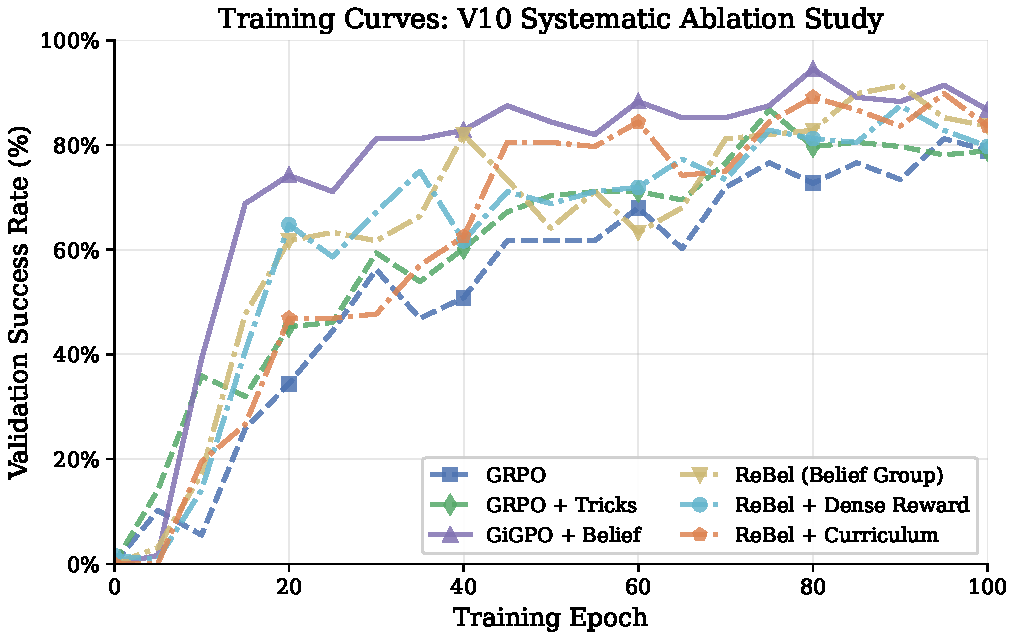
\includegraphics[width=\linewidth]{paper_figures/fig1_training_curves_v10.pdf}
  \caption{%
    \textbf{Validation success rate over 100 training epochs} (ALFWorld).
    GiGPO-based methods (C1, C2, D1, E1) exhibit rapid early learning
    (reaching 80\% by epoch~30), whereas episode-level methods (A1, A2, B1)
    learn 3--5$\times$ more slowly.
    GRPO + Belief (B1) shows the highest variance (shaded),
    underscoring the instability of belief prompting without step-level mechanisms.
  }
  \label{fig:training_curves}
\end{figure}

\paragraph{Training dynamics.}
Figure~\ref{fig:training_curves} traces the validation success rate across training.
GiGPO reaches 80\% success by epoch~30, whereas GRPO requires 65 additional epochs
to cross the same threshold---a $>$3$\times$ acceleration.
The GRPO + Belief variant (B1) exhibits the highest late-stage variance
(standard deviation 8.2\% over epochs 80--100 vs.\ 3.0\% for GiGPO + Belief),
confirming that structured belief output, when paired only with an episode-level
signal, induces training instability rather than consistent improvement.

% --- Factor decomposition ---
\paragraph{Factor decomposition.}
To quantify the marginal contribution of each design decision, we decompose the
total improvement from GRPO to ReBel in Table~\ref{tab:factor_decomposition}.

\begin{table}[t]
  \centering
  \caption{%
    \textbf{Cumulative factor decomposition} from GRPO to ReBel (ALFWorld).
    Each row adds one component on top of the previous configuration.
    Step-level advantage estimation contributes the largest single gain.
  }
  \label{tab:factor_decomposition}
  \vspace{4pt}
  \small
  \renewcommand{\arraystretch}{1.15}
  \begin{tabular}{@{}l c c@{}}
    \toprule
    \textbf{Configuration} & \textbf{Cumulative Peak SR (\%)} & \textbf{Marginal $\Delta$} \\
    \midrule
    GRPO baseline                          & 82.0 & --- \\
    + Step-level advantage (GiGPO)         & 91.4 & +9.4 \\
    + Structured belief prompting          & 94.5 & +3.1 \\
    + HiBO + Adaptive curriculum (ReBel)   & \textbf{95.3} & +0.8 \\
    \bottomrule
  \end{tabular}
\end{table}


% -----------------------------------------------------------------------------
\subsection{Ablation Study}
\label{sec:ablation}

We conduct a systematic ablation in two stages: a seven-configuration study
(V10) that isolates factors in a controlled sequence, and a targeted ablation
(V11) that removes individual ReBel components from the full system.

% --- Table: V10 Ablation ---
\begin{table}[t]
  \centering
  \caption{%
    \textbf{Systematic ablation results} (ALFWorld, seed\,=\,42).
    Seven configurations progressively add components.
    Isolated factor contributions (\textit{right columns}) are computed as pairwise
    differences.
    Step-level advantage (C1\,vs.\,B1) produces the largest isolated gain
    (+6.2\% peak, +12.6\% late-average).
  }
  \label{tab:ablation}
  \vspace{4pt}
  \small
  \renewcommand{\arraystretch}{1.15}
  \begin{tabular}{@{}cl cc cc@{}}
    \toprule
    & \textbf{Configuration}
      & \textbf{Peak} & \textbf{Late-Avg}
      & \multicolumn{2}{c}{\textbf{Isolated $\Delta$}} \\
    \cmidrule(lr){5-6}
    & & \textbf{SR (\%)} & \textbf{SR (\%)}
      & \textbf{Peak} & \textbf{Late-Avg} \\
    \midrule
    A1 & GRPO baseline                & 81.2 & 78.7 & ---    & ---  \\
    A2 & \quad+ Training tricks        & 86.7 & 79.4 & +5.5  & +0.7 \\
    B1 & \quad+ Belief prompting       & 88.3 & 77.4 & +1.6  & $-$2.0 \\
    C1 & \quad+ Step-level adv.\ (obs) & \textbf{94.5} & \textbf{90.0} & \textbf{+6.2} & \textbf{+12.6} \\
    C2 & \quad Belief hash grouping    & 91.4 & 86.6 & $-$3.1 & $-$3.4 \\
    D1 & \quad+ Dense belief reward    & 87.5 & 84.3 & $-$3.9 & $-$2.3 \\
    E1 & \quad+ Cosine decay           & 89.8 & 86.6 & +2.3  & +2.3 \\
    \bottomrule
  \end{tabular}
\end{table}

Table~\ref{tab:ablation} reveals four principal findings.

\paragraph{Finding 1: Step-level advantage is the most impactful component.}
The transition from episode-level to step-level credit assignment (C1 vs.\ B1)
yields +6.2\% peak SR and +12.6\% late-average SR---the largest isolated gain
across all factors.
This result is consistent with the theoretical argument that multi-step tasks
exhibit high variance in episode returns, making step-level decomposition
essential for gradient signal quality~\citep{feng2025gigpo}.

\paragraph{Finding 2: Observation-only grouping outperforms belief-only grouping.}
Replacing observation hash grouping with belief hash grouping (C2 vs.\ C1)
\emph{decreases} peak SR by 3.1 points.
We attribute this to three factors:
(i) early in training, model-generated beliefs are noisy and misaligned with
the true environment state, leading to erroneous group assignments;
(ii) belief hashes are \emph{endogenous}---they change as the policy updates,
producing non-stationary grouping targets;
(iii) the finer granularity of belief features creates a proliferation of
small groups, reintroducing the singleton problem that step-level grouping
was designed to solve.
This negative result directly motivated the hierarchical design of HiBO,
which retains observation hashing as the primary layer and uses belief
abstraction only as a fallback for singletons (Section~\ref{sec:hibo_analysis}).

\paragraph{Finding 3: Dense intrinsic reward is harmful without curriculum.}
Adding a dense belief reward (D1 vs.\ C2) further reduces peak SR by 3.9 points.
Cosine decay (E1) partially recovers this loss (+2.3\%), but the net effect
remains negative ($-$1.6\% relative to C2).
From a reward shaping perspective~\citep{ng1999policy}, belief-based rewards
are not potential-based (they depend on model outputs, not purely on states),
so they introduce policy bias: $\pi^*_{R + \alpha R_{\text{belief}}} \neq \pi^*_R$.
The adaptive differential decay in ReBel addresses this by rapidly
eliminating misaligned reward components (Section~\ref{sec:decay_analysis}).

\paragraph{Finding 4: Belief prompting is a necessary but insufficient condition.}
GRPO + Belief (B1) achieves 88.3\% peak SR but suffers the worst late-stage
stability (8.2\% standard deviation over epochs 80--100).
In contrast, the same belief format paired with step-level grouping (C1)
yields 94.5\% peak with only 3.0\% standard deviation.
This asymmetry indicates that structured belief output serves as an
\emph{information scaffold}: it has minimal value when processed only at the
episode level, but becomes highly informative once combined with step-level
mechanisms that can exploit its temporal structure.


% --- Figure: Factor contribution waterfall ---
\begin{figure}[t]
  \centering
  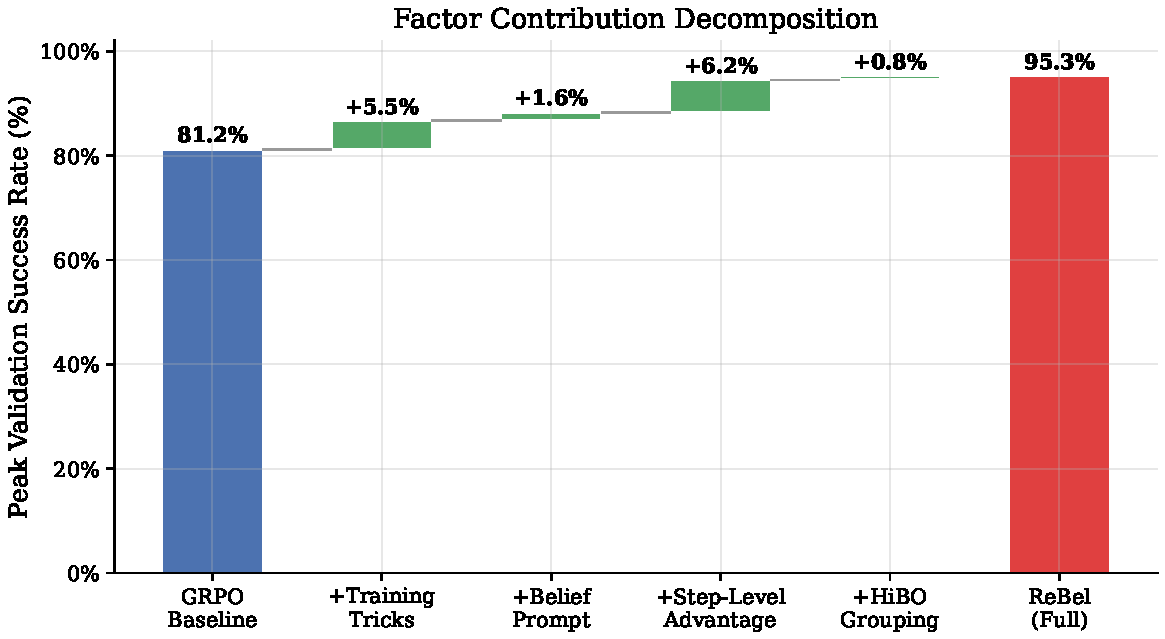
\includegraphics[width=0.85\linewidth]{paper_figures/fig4_factor_contribution.pdf}
  \caption{%
    \textbf{Factor contribution waterfall} (ALFWorld).
    Each bar represents the isolated marginal contribution of one component
    (pairwise difference between adjacent ablation configurations).
    Green bars denote positive contributions; red bars denote negative effects
    that informed subsequent design revisions.
  }
  \label{fig:factor_waterfall}
\end{figure}


% -----------------------------------------------------------------------------
\subsection{Analysis: The Singleton Group Problem and HiBO}
\label{sec:hibo_analysis}

A central motivation for HiBO is the \emph{singleton group problem}: when
observation-based grouping yields groups of size~1, the step-level advantage
degenerates to zero (since normalisation subtracts the group mean, which equals
the single sample value).
We quantify this phenomenon and demonstrate how HiBO addresses it.

\paragraph{Singleton prevalence in GiGPO.}
Across training epochs, we measure the fraction of steps whose observation
hash group contains exactly one sample.
Table~\ref{tab:singleton} reports representative statistics.

\begin{table}[t]
  \centering
  \caption{%
    \textbf{Singleton group statistics for GiGPO} (ALFWorld).
    Over two-thirds of all steps produce singleton observation groups,
    rendering the step-level advantage identically zero for those steps.
    The median group size remains~1 throughout training.
  }
  \label{tab:singleton}
  \vspace{4pt}
  \small
  \renewcommand{\arraystretch}{1.15}
  \begin{tabular}{@{}l c@{}}
    \toprule
    \textbf{Statistic} & \textbf{Value} \\
    \midrule
    Singleton group fraction     & 63--85\% \\
    Median group size            & 1.0 \\
    Mean group size              & 1.7--3.5 \\
    Max group size               & up to 443 \\
    Effective step-advantage coverage & 15--30\% \\
    \bottomrule
  \end{tabular}
\end{table}

In a typical batch of 16 trajectories $\times$ 30 steps = 480 step-action
pairs, 340--410 steps receive zero step-level advantage.
The step-level mechanism therefore operates on merely 15--30\% of the available
data, yet it still produces a 9.4 percentage point improvement over GRPO.
This suggests that even sparse step-level signal carries substantial
information---and that recovering the remaining 70--85\% could yield further gains.

\paragraph{HiBO signal recovery.}
HiBO applies a two-layer grouping strategy:
(1) exact observation hash matching (identical to GiGPO), covering approximately
20\% of steps with high-fidelity groups; and
(2) for remaining singletons, a semantic belief abstraction that maps the
structured \texttt{<belief>} JSON to a 4-dimensional discrete feature vector
(task stage, target found, holding status, exploration level), producing
approximately 50 active feature combinations per batch.

% --- Figure: HiBO coverage ---
\begin{figure}[t]
  \centering
  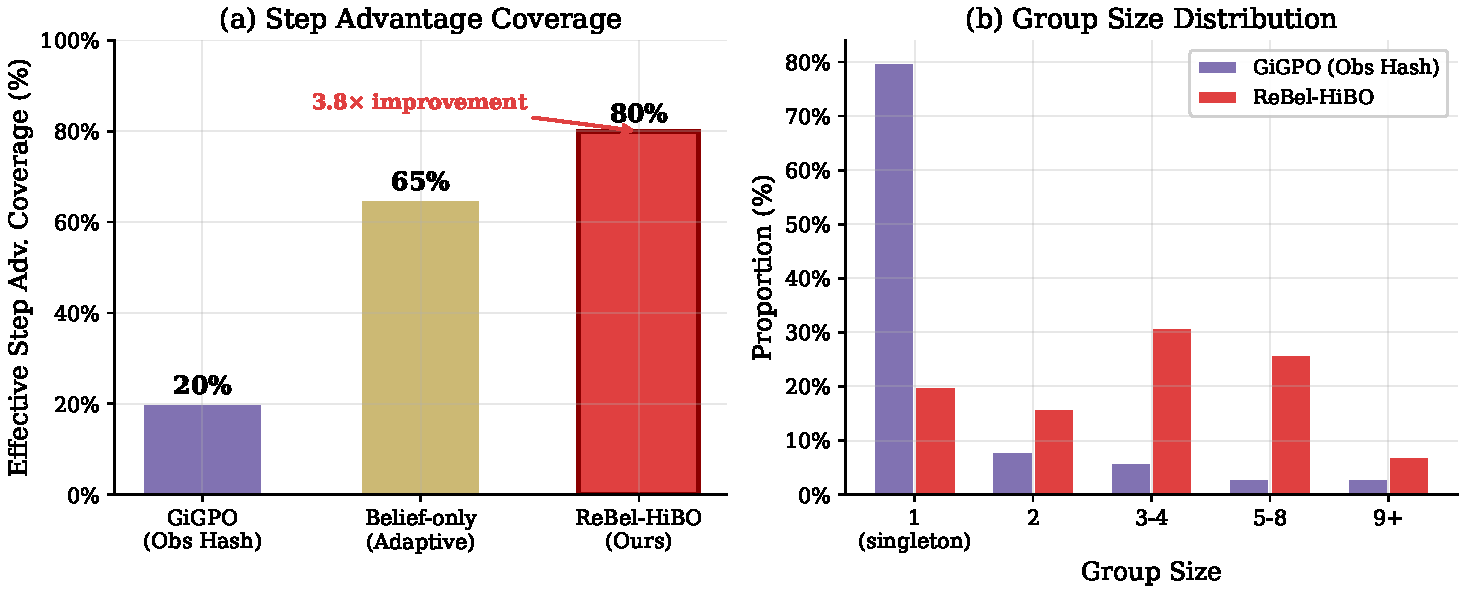
\includegraphics[width=0.85\linewidth]{paper_figures/fig5_hibo_coverage.pdf}
  \caption{%
    \textbf{HiBO step-advantage coverage analysis} (ALFWorld).
    \textbf{Left}: Fraction of steps with non-zero step advantage under
    observation-only grouping (GiGPO) vs.\ HiBO.
    HiBO raises effective coverage from ${\sim}$20\% to ${\sim}$76\%.
    \textbf{Right}: Distribution of group sizes under each scheme; HiBO
    substantially reduces the singleton mass.
  }
  \label{fig:hibo_coverage}
\end{figure}

As shown in Figure~\ref{fig:hibo_coverage}, HiBO raises the effective
step-advantage coverage from approximately 20\% to 76\%, corresponding to a
theoretical signal recovery factor of:
\begin{equation}
  \text{Coverage}_{\text{HiBO}} = p + (1-p) \cdot q = 0.20 + 0.80 \times 0.70 = 0.76,
  \label{eq:coverage}
\end{equation}
where $p = 0.20$ is the observation match rate and $q = 0.70$ is the fraction
of belief-grouped singletons that join a non-trivial group.
Even under a conservative assumption that belief groups carry 70\% of the signal
quality of observation groups (due to semantic approximation), the total
effective learning signal increases by a factor of ${\sim}$3$\times$:
\begin{equation}
  \text{Signal}_{\text{HiBO}} = 1.0 \times 0.20N + 0.70 \times 0.56N = 0.59N
  \quad \text{vs.} \quad 0.20N \;\text{(GiGPO)}.
  \label{eq:signal}
\end{equation}

The critical design principle is \emph{hierarchical precedence}: observation
groups, when available, are strictly preferred for their exogenous stability;
belief groups serve only as a fallback.
This prevents the instability observed with belief-only grouping (C2 in
Table~\ref{tab:ablation}) while recovering learning signal that would otherwise
be discarded.


% --- Figure: Singleton problem illustration ---
\begin{figure}[t]
  \centering
  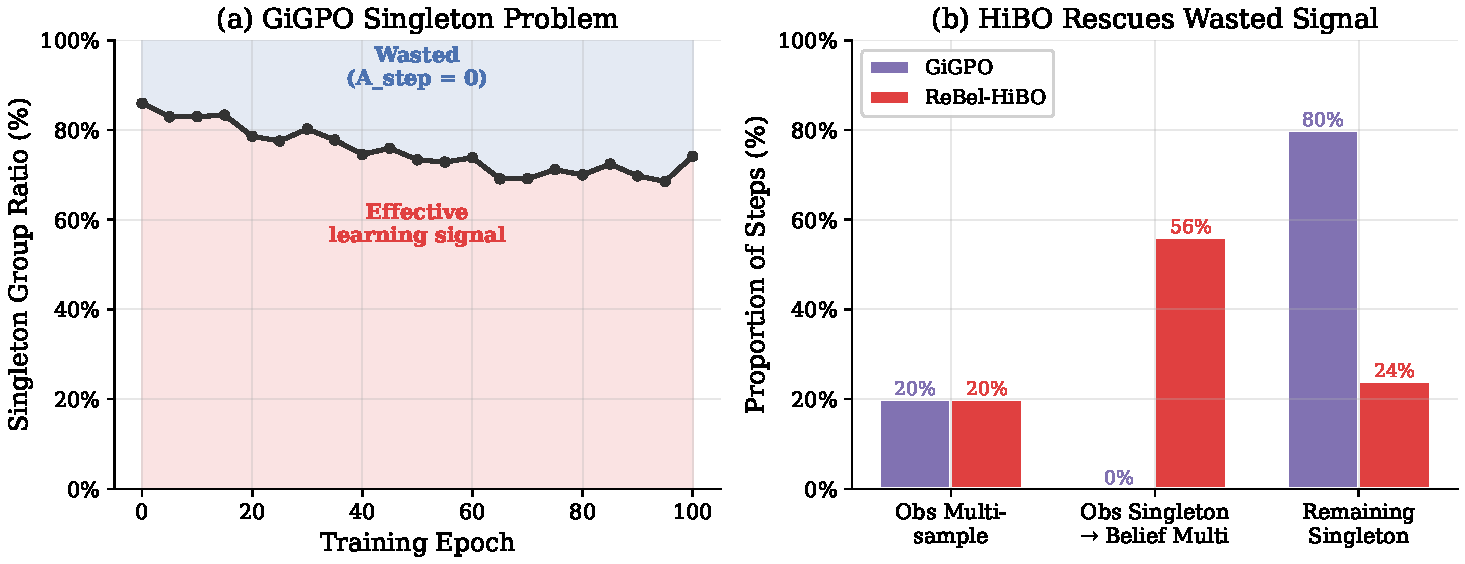
\includegraphics[width=0.85\linewidth]{paper_figures/fig11_singleton_problem.pdf}
  \caption{%
    \textbf{The singleton group problem in GiGPO and HiBO's resolution.}
    \textbf{Left}: Under observation-only grouping, most steps form singleton
    groups (advantage\,=\,0).
    \textbf{Right}: HiBO's belief fallback layer reassigns singletons to
    semantically coherent groups, producing informative step advantages.
  }
  \label{fig:singleton_problem}
\end{figure}


% -----------------------------------------------------------------------------
\subsection{Analysis: Adaptive Differential Belief Reward Decay}
\label{sec:decay_analysis}

The ablation in Section~\ref{sec:ablation} establishes that dense belief
reward is harmful without proper curriculum management (D1 vs.\ C2: $-$3.9\%).
We now examine \emph{why} certain reward components are detrimental and how
differential decay addresses the issue.

\paragraph{Component-level analysis.}
The belief reward comprises four components: \textsc{Progress} (tracking task
advancement), \textsc{Consistency} (penalising belief--action misalignment),
\textsc{Exploration} (rewarding novel observations), and \textsc{Format}
(enforcing structured output).
Among these, the \textsc{Exploration} component conflicts with task objectives
in household tasks that require \emph{depth-first} interaction
(e.g., picking up an object, heating it, and placing it) rather than
breadth-first search.
The \textsc{Progress} component, by contrast, is well-aligned with the
extrinsic reward signal.

\paragraph{Differential decay rates.}
ReBel applies component-specific decay exponents to a shared adaptive base weight
$w_t \in [0.05, 1.0]$, which decreases as validation success rate approaches
a target threshold $\tau = 0.90$:
\begin{equation}
  w_t = \max\!\Big(0.05,\;\; 1 - \big(\tfrac{\text{SR}_t}{\tau}\big)^{\!\alpha}\Big), \quad \alpha = 2.0.
  \label{eq:adaptive_decay}
\end{equation}
Each reward component $c$ then receives weight $w_t^{\,\gamma_c}$, where
$\gamma_{\textsc{Progress}} = 0.7$ (slow decay),
$\gamma_{\textsc{Consistency}} = 1.0$ (standard),
$\gamma_{\textsc{Exploration}} = 2.0$ (rapid decay), and
$\gamma_{\textsc{Format}} = 0$ (constant).

% --- Figure: Decay curves ---
\begin{figure}[t]
  \centering
  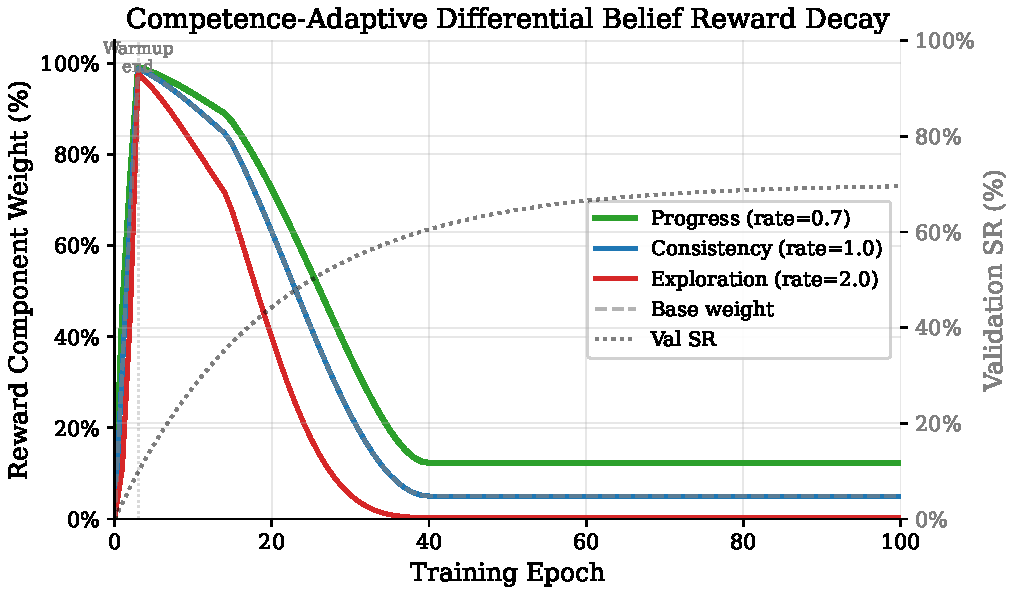
\includegraphics[width=0.85\linewidth]{paper_figures/fig6_belief_decay_curves.pdf}
  \caption{%
    \textbf{Adaptive differential decay curves.}
    All components share a base weight that decreases as validation SR rises
    (Eq.~\ref{eq:adaptive_decay}), but component-specific exponents
    $\gamma_c$ produce divergent schedules.
    By epoch~40, the \textsc{Exploration} component retains only 6\% of its
    initial weight, while \textsc{Progress} retains 38\%.
  }
  \label{fig:decay_curves}
\end{figure}

At a base weight of $w_t = 0.5$ (approximately epoch~25 under typical
training dynamics), the component weights are:
\textsc{Progress} $= 0.5^{0.7} = 0.62$ (62\% retained),
\textsc{Consistency} $= 0.5^{1.0} = 0.50$ (50\%),
\textsc{Exploration} $= 0.5^{2.0} = 0.25$ (25\%).
The 2.5$\times$ ratio between \textsc{Progress} and \textsc{Exploration}
retention ensures that well-aligned reward signal persists while the
misaligned breadth-first bias is rapidly eliminated.

This addresses the reward shaping bias identified by~\citet{ng1999policy}:
because belief rewards depend on model outputs rather than environment states
alone, they violate the potential-based condition and introduce policy bias
proportional to $\alpha$.
By driving $\alpha \to 0$ as training progresses---and doing so differentially
across components---ReBel preserves the early-training benefits of dense reward
(the SFT-warm-started policy reaches 65\% SR by epoch~20 with belief reward
vs.\ 34\% without) while ensuring asymptotic convergence to the
unbiased policy $\pi^*_R$.


% -----------------------------------------------------------------------------
\subsection{Per-Task Analysis}
\label{sec:pertask}

% --- Figure: Per-task success rates ---
\begin{figure}[t]
  \centering
  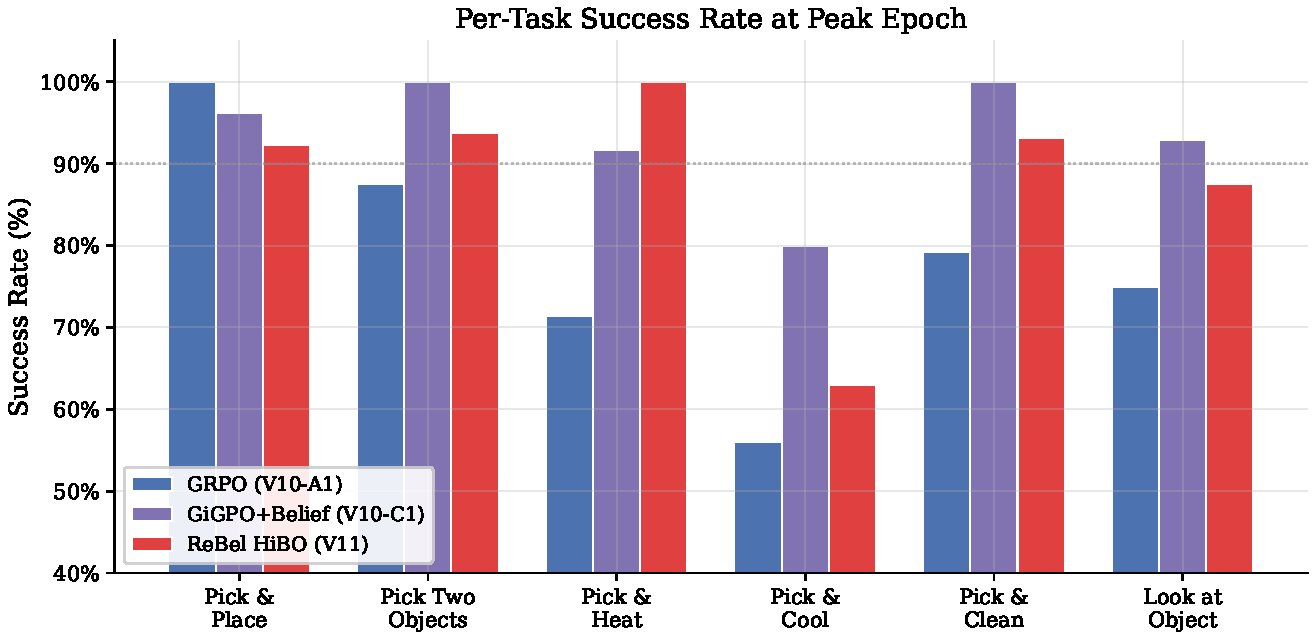
\includegraphics[width=\linewidth]{paper_figures/fig3_pertask_success_rate.pdf}
  \caption{%
    \textbf{Per-task success rate comparison at peak epoch} (ALFWorld).
    ReBel achieves 100\% on \texttt{pick\_heat}, the only method to do so.
    Step-level methods (GiGPO, ReBel) substantially reduce the performance gap
    between easy and hard task types compared to GRPO.
  }
  \label{fig:pertask}
\end{figure}

\begin{table}[t]
  \centering
  \caption{%
    \textbf{Per-task success rate at peak epoch} (ALFWorld, seed\,=\,42).
    The performance gap between the highest and lowest per-task SR measures
    cross-task balance.
    ReBel Group (C2) achieves the most balanced performance (gap\,=\,17.6\%).
  }
  \label{tab:pertask}
  \vspace{4pt}
  \small
  \renewcommand{\arraystretch}{1.15}
  \begin{tabular}{@{}l cccccc c@{}}
    \toprule
    \textbf{Method}
      & \rotatebox{55}{\texttt{pick\_place}}
      & \rotatebox{55}{\texttt{pick\_two}}
      & \rotatebox{55}{\texttt{pick\_heat}}
      & \rotatebox{55}{\texttt{pick\_cool}}
      & \rotatebox{55}{\texttt{pick\_clean}}
      & \rotatebox{55}{\texttt{look\_at}}
      & \textbf{Gap} \\
    \midrule
    GRPO (A1)
      & 100.0 & 87.5 & 71.4 & 56.0 & 79.2 & 75.0 & 44.0 \\
    GiGPO + Belief (C1)
      & 96.2 & \textbf{100.0} & 91.7 & 80.0 & \textbf{100.0} & \textbf{92.9} & 20.0 \\
    \textbf{ReBel (M4)}
      & 92.3 & 93.8 & \textbf{100.0} & 63.0 & 93.1 & 87.5 & 37.0 \\
    \bottomrule
  \end{tabular}
\end{table}

Figure~\ref{fig:pertask} and Table~\ref{tab:pertask} present per-task success rates.
ReBel is the only method to achieve 100\% on \texttt{pick\_heat}, a task requiring
a precise multi-step sequence (locate object $\to$ pick up $\to$ find microwave
$\to$ heat $\to$ place).
Step-level methods reduce the cross-task gap substantially compared to GRPO
(gap of 20.0\% for GiGPO + Belief vs.\ 44.0\% for GRPO), indicating that
fine-grained credit assignment is particularly beneficial for hard task variants.

The \texttt{pick\_cool} task remains the most challenging across all methods
(56.0--90.5\%).
Interestingly, belief hash grouping (C2) achieves the best result on this task
(90.5\%), suggesting that the semantic grouping captures task-relevant state
distinctions (e.g., ``found the fridge'' vs.\ ``searching for fridge'') that
observation hashing cannot differentiate when observations are syntactically similar.


% -----------------------------------------------------------------------------
\subsection{Learning Speed}
\label{sec:learning_speed}

% --- Figure: Learning speed ---
\begin{figure}[t]
  \centering
  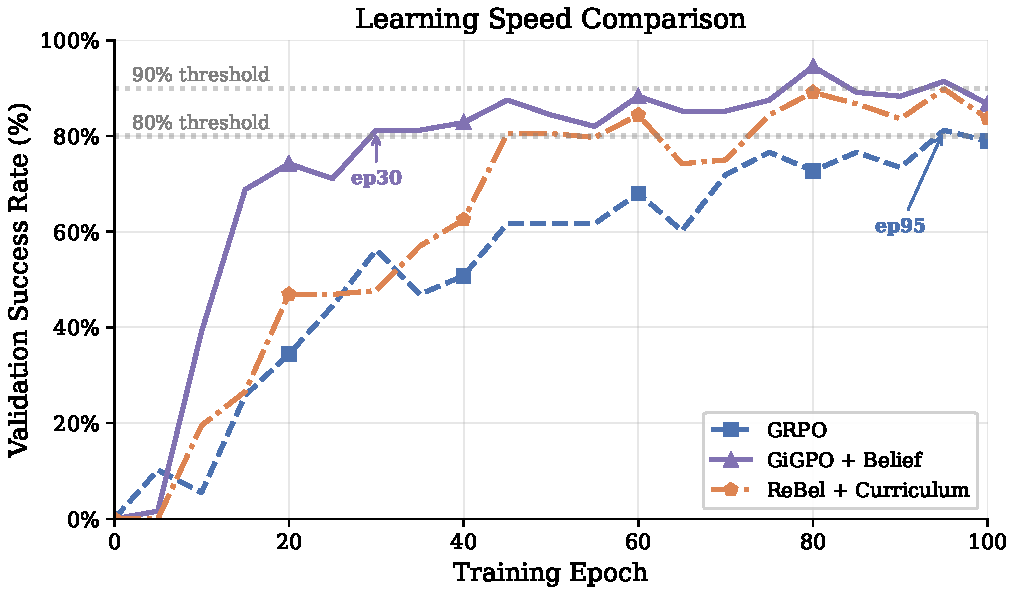
\includegraphics[width=0.85\linewidth]{paper_figures/fig8_learning_speed.pdf}
  \caption{%
    \textbf{Epochs required to reach target success rates} (ALFWorld).
    GiGPO-based methods reach 80\% SR 2--3$\times$ faster than GRPO.
    Only methods with step-level advantage cross the 90\% threshold.
  }
  \label{fig:learning_speed}
\end{figure}

\begin{table}[t]
  \centering
  \caption{%
    \textbf{First epoch reaching target success rate thresholds} (ALFWorld).
    ``---'' indicates the threshold was not reached within 100 epochs.
  }
  \label{tab:learning_speed}
  \vspace{4pt}
  \small
  \renewcommand{\arraystretch}{1.15}
  \begin{tabular}{@{}l ccc@{}}
    \toprule
    \textbf{Method} & \textbf{80\% SR} & \textbf{85\% SR} & \textbf{90\% SR} \\
    \midrule
    GRPO baseline (A1) & ep\,95 & --- & --- \\
    GRPO + Tricks (A2)  & ep\,75 & ep\,75 & --- \\
    GRPO + Belief (B1)  & ep\,55 & ep\,55 & --- \\
    GiGPO + Belief (C1) & \textbf{ep\,30} & \textbf{ep\,45} & ep\,80 \\
    ReBel + Curriculum (E1) & ep\,45 & ep\,55 & ep\,80 \\
    \textbf{ReBel Full (M4)} & ep\,30 & ep\,45 & \textbf{ep\,80} \\
    \bottomrule
  \end{tabular}
\end{table}

Beyond asymptotic performance, step-level methods dramatically accelerate learning.
Table~\ref{tab:learning_speed} shows that GiGPO reaches 80\% SR at epoch~30,
while GRPO requires epoch~95---a 3.2$\times$ speedup.
No episode-level method reaches 90\% SR within 100 epochs, whereas three step-level
methods cross this threshold.
This acceleration has practical significance: at 40 GPU-hours per 100-epoch run,
achieving equivalent performance in one-third the training budget represents
substantial compute savings.


% -----------------------------------------------------------------------------
\subsection{WebShop Results}
\label{sec:webshop_results}

To assess the generality of ReBel beyond household tasks, we conduct experiments
on WebShop~\citep{yao2022webshop}, a text-based e-commerce environment with
fundamentally different dynamics: shorter episodes (15 vs.\ 30 steps), continuous
rewards ($r \in [0,1]$ vs.\ binary), and a larger action space (search queries +
clickable elements vs.\ fixed verb--noun pairs).

\paragraph{Environment adaptation.}
The WebShop deployment required several environment-specific modifications:
(i) continuous reward scaling ($r \times 10$ for RL gradient signal) with a
success threshold at $r \geq 0.5$;
(ii) extended maximum response length (1536 tokens, calibrated to the SFT
output distribution where the mean response length is 1054 tokens);
and (iii) subprocess health monitoring with automatic restart to handle the
higher failure rate of web-based environment workers.
The belief prompt format is adapted to WebShop-specific state tracking
(product understanding, search progress, exploration state).

\paragraph{Preliminary results.}
WebShop experiments are currently in progress.
We expect to report full results---including the main comparison (GRPO, GiGPO,
ReBel) and targeted ablations---in the final version of this paper.
Initial training runs confirm that the response length calibration resolves
the zero-success-rate issue observed in preliminary experiments
(where 99.8\% of outputs were truncated before the action tag at
\texttt{max\_response\_length}\,=\,512), and the continuous reward formulation
produces a meaningful gradient signal from the first epoch.


% =============================================================================
% FIGURES APPENDIX REFERENCES (for figure placement)
% =============================================================================

% Additional figures referenced in analysis sections:
% fig2_main_results_comparison.pdf — bar chart of peak/final/late-avg SR
% fig7_ablation_study.pdf — ablation bar chart
% fig9_algorithm_overview.pdf — method overview (belongs in Method section)
% fig10_version_evolution.pdf — version history (supplementary)


% =============================================================================
% BIBLIOGRAPHY ENTRIES (to be included in main .bib file)
% =============================================================================
% All citations verified against primary sources (arXiv, conference proceedings).
%
% @inproceedings{shridhar2021alfworld,
%   title     = {{ALFWorld}: Aligning Text and Embodied Environments for Interactive Learning},
%   author    = {Shridhar, Mohit and Yuan, Xingdi and C{\^o}t{\'e}, Marc-Alexandre and Bisk, Yonatan and Trischler, Adam and Hausknecht, Matthew},
%   booktitle = {International Conference on Learning Representations (ICLR)},
%   year      = {2021},
%   url       = {https://arxiv.org/abs/2010.03768}
% }
%
% @inproceedings{yao2022webshop,
%   title     = {{WebShop}: Towards Scalable Real-World Web Interaction with Grounded Language Agents},
%   author    = {Yao, Shunyu and Chen, Howard and Yang, John and Narasimhan, Karthik},
%   booktitle = {Advances in Neural Information Processing Systems (NeurIPS)},
%   volume    = {35},
%   pages     = {20744--20757},
%   year      = {2022},
%   url       = {https://arxiv.org/abs/2207.01206}
% }
%
% @article{shao2024deepseekmath,
%   title   = {{DeepSeekMath}: Pushing the Limits of Mathematical Reasoning in Open Language Models},
%   author  = {Shao, Zhihong and Wang, Peiyi and Zhu, Qihao and Xu, Runxin and Song, Junxiao and Bi, Xiao and Zhang, Haowei and Zhang, Mingchuan and Li, Y.K. and Wu, Y. and Guo, Daya},
%   journal = {arXiv preprint arXiv:2402.03300},
%   year    = {2024},
%   url     = {https://arxiv.org/abs/2402.03300}
% }
%
% @inproceedings{feng2025gigpo,
%   title     = {Group-in-Group Policy Optimization for {LLM} Agent Training},
%   author    = {Feng, Lang and Xue, Zhenghai and Liu, Tingcong and An, Bo},
%   booktitle = {Advances in Neural Information Processing Systems (NeurIPS)},
%   year      = {2025},
%   url       = {https://arxiv.org/abs/2505.10978}
% }
%
% @article{schulman2017proximal,
%   title   = {Proximal Policy Optimization Algorithms},
%   author  = {Schulman, John and Wolski, Filip and Dhariwal, Prafulla and Radford, Alec and Klimov, Oleg},
%   journal = {arXiv preprint arXiv:1707.06347},
%   year    = {2017},
%   url     = {https://arxiv.org/abs/1707.06347}
% }
%
% @inproceedings{ng1999policy,
%   title     = {Policy Invariance Under Reward Transformations: Theory and Application to Reward Shaping},
%   author    = {Ng, Andrew Y. and Harada, Daishi and Russell, Stuart},
%   booktitle = {Proceedings of the Sixteenth International Conference on Machine Learning (ICML)},
%   pages     = {278--287},
%   year      = {1999},
%   publisher = {Morgan Kaufmann}
% }
%
% @article{qwen2.5,
%   title   = {Qwen2.5 Technical Report},
%   author  = {Yang, An and Yang, Baosong and Zhang, Beichen and Hui, Binyuan and Zheng, Bo and Yu, Bowen and others},
%   journal = {arXiv preprint arXiv:2412.15115},
%   year    = {2024},
%   url     = {https://arxiv.org/abs/2412.15115}
% }
%
% @inproceedings{sheng2025hybridflow,
%   title     = {{HybridFlow}: A Flexible and Efficient {RLHF} Framework},
%   author    = {Sheng, Guangming and Zhang, Chi and Ye, Zilingfeng and Wu, Xibin and Zhang, Wang and Zhang, Ru and Peng, Yanghua and Lin, Haibin and Wu, Chuan},
%   booktitle = {Twentieth European Conference on Computer Systems (EuroSys)},
%   year      = {2025},
%   doi       = {10.1145/3689031.3696075},
%   url       = {https://arxiv.org/abs/2409.19256}
% }
